\documentclass{article}

\usepackage{../template}

\usepackage{cleveref}
\usetikzlibrary{knots}

\title{05: Wielomian Jonesa\\ węzłów alternujących}
\author{Weronika Jakimowicz}
\date{27.03.2024}

\declaretheorem[
   name=Fakt,
   numbered=no,
   style=uwagi-lematy
]{fuck}
 
\renewenvironment{proof}{{\bfseries\color{orange} Dowód}$ $\newline}{
  \begin{flushright}\includegraphics[width=30pt]{Donald_Duck.png}\end{flushright}$ $\newline
}

\begin{document}
\maketitle

\def\dupa{\textwidth - 4cm}
\begin{tikzpicture}[overlay, remember picture]
  \foreach \i in {0,..., 10} {
    \pgfmathparse{Mod(\i,2)==0?1:0)}
    \ifnum\pgfmathresult>0 
      \node at (4-1*\i,4.7) {\includegraphics[width=1cm]{kaczusia.png}};
    \else 
      \node at (4-1*\i, 4.3) {\includegraphics[width=1cm]{kaczusia.png}};
    \fi
  }
  \foreach \i in {0,..., 10} {%\node at (\dupa + \i*1cm, 4.5) {\includegraphics[width=1cm]{kaczusia.png}};
    \pgfmathparse{Mod(\i,2)==0?1:0)}
    \ifnum\pgfmathresult>0 
      \node at (\dupa+\i*1cm,4.7) {\includegraphics[width=1cm]{kaczusia.png}};
    \else 
      \node at (\dupa+\i*1cm, 4.3) {\includegraphics[width=1cm]{kaczusia.png}};
    \fi
  }
\end{tikzpicture}

Mówimy, że diagram regularny $D$ węzła $K$ jest alternujący, jeśli poruszając dowolny punkt $P\in D$ wzdłuż $D$, ciągle w jedną stronę, będziemy na zmianę pokonywać skrzyżowania górą i dołem.

\begin{deff}[węzeł alternujący]
  Węzeł $K$ jest alternujący, jeśli posiada przynajmniej jeden diagram alternujący.
\end{deff}

Najprostszy (o najmniejszej liczbie skrzyżowań) węzeł niealternujący to np. $8_{19}$ (ale też $8_{20}$ i $8_{21}$), który widać na \cref{diagram 8 19}. Do pokazania, że naprawdę nie kłamię jeśli chodzi o jego niealternującą naturę, wrócimy przy okazji powierzchni Seiferta i \emph{sygnatury węzła}.
\begin{figure}[h]\centering
  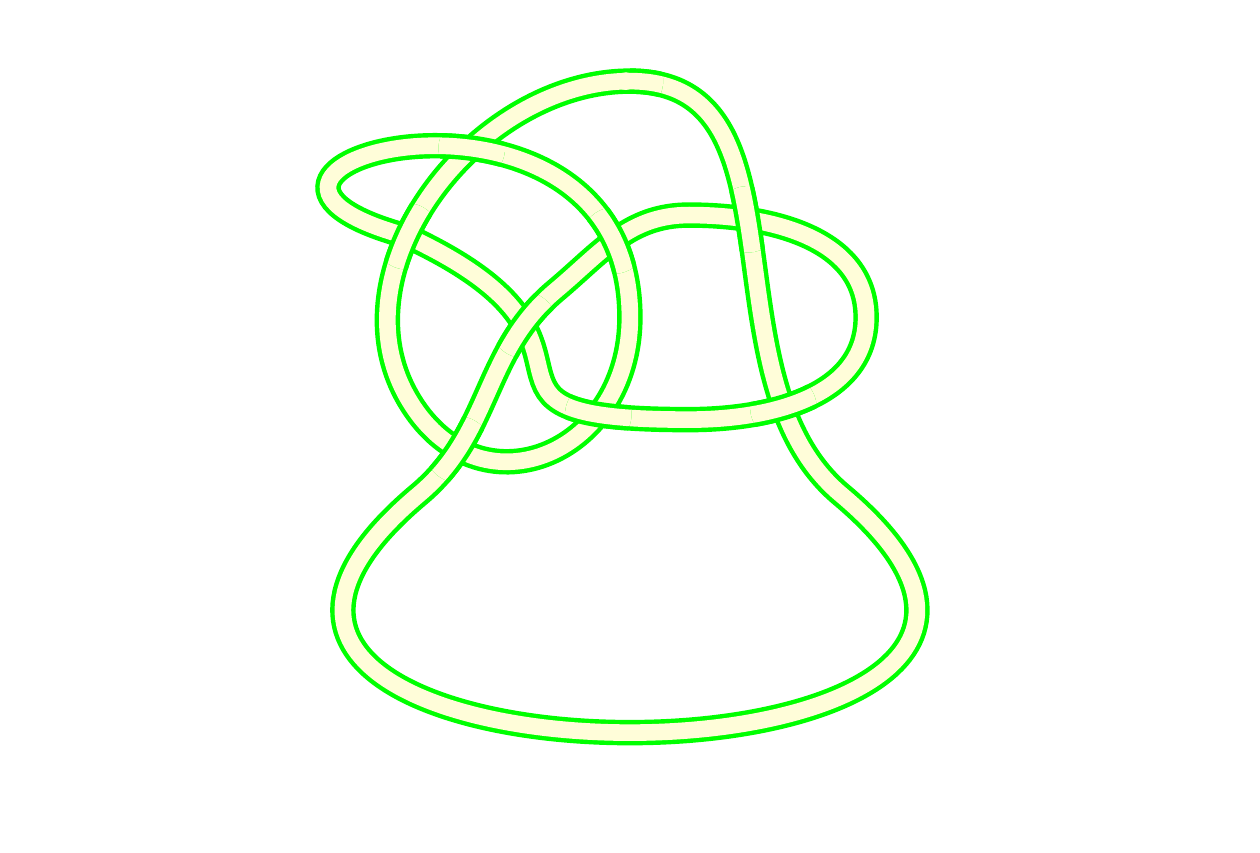
\begin{tikzpicture}
    \coordinate (a0) at (0,0);
    \coordinate (a1) at (90:3);
    \coordinate (a2) at (-40:3.5);
    \coordinate (a3) at (220:3.5);
    \coordinate (a4) at (160:1);
    \coordinate (a5) at (60:1.5);
    \coordinate (a6) at (0:3);
    \coordinate (a7) at (-60:1.5);
    \coordinate (a8) at (160:3);
    \coordinate (a9) at (200:3);

    %\foreach \i in {0,...,9} \fill (a\i) circle (3pt);
      
    \begin{knot}[
      clip width=2,
%      draft mode=crossings,
      consider self intersections,
      ignore endpoint intersections=false,
      flip crossing=2,
      flip crossing=6,
      flip crossing=8,
      line join=round,
      background color=white,
        only when rendering/.style={
        draw=green,
        ultra thick,
        double=yellow!15,
        double distance=6pt,
        %line cap=round,
      }
      ]
        \strand[thick] 
        (a1) to[out=0, in=140]
        (a2) to [out= -40, in=-140, looseness=3]
        (a3) to [out=40, in=-140]
        (a4) to [out=40, in=180]
        (a5) to [out=0, in=90]
        (a6) to [out=-90, in=0]
        (a7) to [out=180, in=-25, looseness=2]
        (a8) to [out=165, in=90, looseness=3]
        (a0) to [out=-90, in=-60, looseness=1.5]
        (a9) to [out=120, in=180]
        (a1);
    \end{knot}
    \fill[yellow!15] (91:3) circle (3.2pt);
  \end{tikzpicture}
  \caption{\label{diagram 8 19}Przykładowy diagram węzła $8_{19}$.}
\end{figure}

\begin{fuck}[alternująca suma spójna]
  Jeśli $K_1$ i $K_2$ są węzłami alternującymi o alternujących diagramach mających odpowiednio $n_1$ i $n_2$ skrzyżowań, to ich suma spójna $K_1\#K_2$ ma diagram alternujący o dokładnie $(n_1+n_2)$ skrzyżowaniach.
\end{fuck}

\begin{proof}
  Wiemy, że "na zewnątrz" węzła $K_1$ istnieje segment, pod którym przechodzi dokładnie jeden inny segment. Tak samo w przypadku diagramu $K_2$. Mamy dwie opcje:
  \begin{figure}[h]\centering
    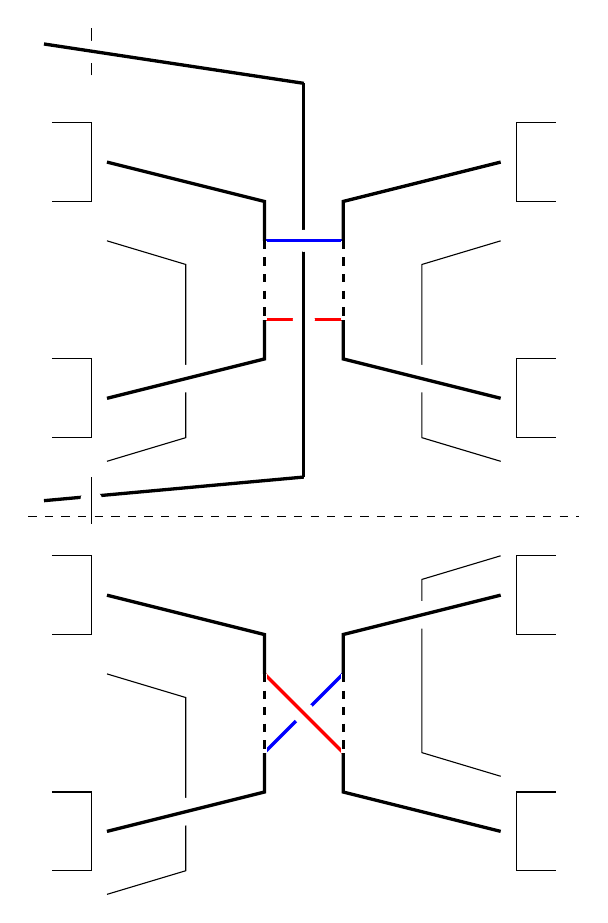
\begin{tikzpicture}
      \draw (-.2, 1.1)--(-.2, 1.7);
      \fill[white] (-.2, 1.4) circle (4pt);
      \draw[very thick] (2.5, -1.5)--(2.5, 1);
      \fill[white](2.5, -1) circle (4pt);
      \draw[very thick, blue] (2, -1)--(3, -1);
      \draw[very thick, red] (2, -2)--(3, -2);
      \fill[white] (2.5, -2) circle (4pt);
      \draw[very thick] (2.5, -4)--(2.5, -1.5);
      \draw[very thick] (2.5, -4)--(-0.8, -4.3);
      \fill[white] (-0.2, -4.3) circle (4pt);
      \draw[very thick] (2.5, 1)--(-0.8, 1.5);
      \draw (-.2, -4)--(-0.2, -4.6);
      
      \draw (-0.7, 0.5)--(-0.2, 0.5)--(-0.2, -0.5)--(-0.7, -0.5);
      \draw (0, -1)--(1, -1.3)--(1, -3.5)--(0, -3.8);
      \fill[white] (1, -2.75) circle (5pt);
      \draw[very thick] (0,0)--(2, -0.5)--(2, -2.5)--(0, -3);
      \draw (-0.7, -2.5)--(-0.2, -2.5)--(-0.2, -3.5)--(-0.7, -3.5);

      \draw (5, -1)--(4, -1.3)--(4, -3.5)--(5, -3.8);
      \fill[white] (4, -2.75) circle (5pt);
      \draw[very thick] (5, 0)--(3, -0.5)--(3, -2.5)--(5, -3);
      \draw (5.7, 0.5)--(5.2, 0.5)--(5.2, -0.5)--(5.7, -0.5);
      \draw (5.7, -2.5)--(5.2, -2.5)--(5.2, -3.5)--(5.7, -3.5);

      \draw[ultra thick, white] (2, -1)--(2, -2);
      \draw[ultra thick, white] (3, -1)--(3, -2);

      \draw[very thick, dashed] (2, -1)--(2, -2);
      \draw[very thick, dashed] (3, -1)--(3, -2);
      
      \draw[dashed] (-1, -4.5)--(6, -4.5);

      \begin{scope}[shift={(0, -5.5)}]
        \draw[very thick, blue] (2, -2)--(3, -1);
        \fill[white] (2.5, -1.5) circle (4pt);
        \draw[very thick, red] (2, -1)--(3, -2);
        
        \draw (-0.7, 0.5)--(-0.2, 0.5)--(-0.2, -0.5)--(-0.7, -0.5);
        \draw (0, -1)--(1, -1.3)--(1, -3.5)--(0, -3.8);
        \fill[white] (1, -2.75) circle (5pt);
        \draw[very thick] (0,0)--(2, -0.5)--(2, -2.5)--(0, -3);
        \draw (-0.7, -2.5)--(-0.2, -2.5)--(-0.2, -3.5)--(-0.7, -3.5);

        \draw (5, 0.5)--(4, 0.2)--(4, -2)--(5, -2.3);
        \fill[white] (4, -.25) circle (5pt);
        \draw[very thick] (5, 0)--(3, -0.5)--(3, -2.5)--(5, -3);
        \draw (5.7, 0.5)--(5.2, 0.5)--(5.2, -0.5)--(5.7, -0.5);
        \draw (5.7, -2.5)--(5.2, -2.5)--(5.2, -3.5)--(5.7, -3.5);

        \draw[ultra thick, white] (2, -1)--(2, -2);
        \draw[very thick, dashed] (2, -1)--(2, -2);
        
        \draw[ultra thick, white] (3, -1)--(3, -2);
        \draw[very thick, dashed] (3, -1)--(3, -2);
      \end{scope}
    \end{tikzpicture}
  \end{figure}
\end{proof}

\end{document}
